
\section{Galactic Chemical Evolution Models}
\label{outflows:sec:gce}
\begin{itemize}

	\item We now construct GCE models to understand the origin of the radial
	age and metallicity gradients characterized
	in~\S~\ref{outflows:sec:empirical}.
	To this end, we construct models describing the Galaxy disk as a series of
	one-zone models like those in Chapters~\ref{starbursts} and~\ref{dga} and
	multi-ring models like those in Chapters~\ref{migration} and~\ref{ohno}.
	Though similar, the former does not incorporate mixing of stellar
	populations while the latter does.
	We also extend these models to incorporate radial gas
	flows~\citep[e.g.,][]{Lacey1985, Bilitewski2012}.

\end{itemize}

\subsection{One-Zone Models}
\label{outflows:sec:gce:onezone}

\begin{itemize}

	\item The fundamental assumption of one-zone GCE models is instantaneous
	mixing of newly produced metals in the star-forming ISM.
	In the presence of accretion, star formation, and outflows, the rate of
	change of the ISM gas mass~$M_g$ can be expressed as
	\begin{equation}\begin{split}
	\dot{M}_g &= \dot{M}_\text{in} - \dot{M}_\star - \dot{M}_\text{out} +
	\dot{M}_r
	\\
	&\approx \dot{M}_\text{in} - \dot{M}_\star(1 + \eta - r),
	\end{split}\end{equation}
	where~$\dot{M}_\text{in}$ is the accretion rate,~$\dot{M}_\star$ is the
	SFR,~$\eta \equiv \dot{M}_\text{out} / \dot{M}_\star$ is the
	``mass-loading factor'' parameterizing outflows, and
	$r = \dot{M}_\star / \dot{M}_r$ is a parameter describing the return of
	stellar envelopes back to the ISM.
	Although recycling rates in detail depend on the initial-final mass
	relation {\color{red} (refs)}, the mass-lifetime relation {\color{red}
	(refs)}, and the IMF {\color{red} (refs)}, recycling in general is quite
	fast for young stellar populations but then slows considerably due to the
	steep nature of the mass-lifetime relation.
	\citet{Weinberg2017b} demonstrate that a constant value of~$r = 0.4$
	($0.2$) for a~\citet{Kroupa2001}~\citep{Salpeter1955} IMF is a sufficiently
	accurate approximation for GCE models.

	\item Assuming infalling gas to be zero metallicity, the rate of a change
	of the mass of some element~$x$ in the ISM is given by
	\begin{equation}
	\dot{M}_x = \sum_i \dot{M}_{x,i} - Z_x \dot{M}_\star
	\left(1 + \eta - r\right),
	\end{equation}
	where~$Z_x = M_x / M_g$ is the mass fraction of~$x$ in the ISM
	and~$\sum_i \dot{M}_{x,i}$ generically accounts for enrichment channels
	such as core collapse supernovae (CCSNe), Type Ia supernovae (SNe Ia),
	asymptotic giant branch (AGB) stars, etc. which may produce~$x$ in some
	significant amount.
	In the case of O and Mg, there are arguments from both theoretical
	\citep[e.g.,][]{Andrews2017, Limongi2018} and empirical
	\citep{Griffith2019, Griffith2022, Weinberg2019, Weinberg2022}
	perspectives suggesting that their population-averaged yields are dominated
	by massive stars with a metallicity-independent yield.
	In this case, the above expression reduces to
	\begin{equation}
	\dot{M}_x \approx \ycc{$x$} \dot{M}_\star - Z_x \dot{M}_\star
	\left(1 + \eta - r\right),
	\end{equation}
	where~$\ycc{$x$}$ is the yield of~$x$.
	This expression retains the approximations from {\color{red} previous
	chapters} that enrichment from CCSNe occurs instantaneously after a single
	stellar population's formation, which is valid as long as the timescales of
	galaxy evolution are much longer than the lifetimes of massive stars.

	\item \citet{Weinberg2017b} demonstrate that the first-order details of the
	enrichment history in the ISM are determined by~$\eta$ and the star
	formation efficiency timescale~$\tau_\star \equiv M_g / \dot{M}_\star$.
	In the absence of sudden events such as bursts in star formation
	\citep[e.g.,][]{Johnson2020}, the detailed form of the SFH has minimal
	impact on the shape of the evolutionary track through chemical space
	(e.g., the~\afe-\feh~plane), with that information instead encoded in the
	density of stars along the track.
	However, in the absence of outflows (i.e.,~$\eta = 0$), then the shape of
	the SFH has a stronger effect, and radial flows have a stronger effect.
	{\color{red} Some short discussion on why~$\eta = 0$ versus~$\eta \neq 0$
	is interesting, potentially just referencing the discussion in the
	introduction}.

	\item {\color{red} Speaking of radial flows and Segways!}
	Under the approximation that all of the gas in some ring flows
	inward or outward with a single velocity~$v_R$, we demonstrate in
	Appendix~\ref{outflows:sec:coefficients-derivation} that the rate of change
	of the mass of some element~$x$ due solely to this process can be expressed
	as
	\begin{equation}
	\dot{M}_{x,\flow} = Z_x \dot{M}_\star \mu_\flow,
	\end{equation}
	where~$\mu_\flow$ is a unitless coefficient given by
	\begin{equation}
	\mu_\flow \equiv -\tau_\star v_R
	\left(\frac{1}{R} - \frac{1}{R_g} - \frac{1}{R_x}\right).
	\end{equation}
	$R_g$ is the scale radius of the gas disk, and~$R_x \equiv
	-(\grad{X} \ln 10)^{-1}$ is the scale radius of the exponential gradient
	in~$Z_x$ implied by a linear gradient in [X/H].

	\item Similarly, the rate of change of the ISM mass due to radial flows is
	given by
	\begin{equation}
	\dot{M}_{g,\flow} = \dot{M}_\star \gamma_\flow,
	\end{equation}
	where~$\gamma_\flow$ is given by
	\begin{equation}
	\gamma_\flow \equiv -\tau_\star v_R
	\left(\frac{1}{R} - \frac{1}{R_g}\right)
	= \mu_\flow - \frac{\tau_\star v_R}{R_x}.
	\end{equation}

	\item The coefficients~$\mu_\flow$ and~$\gamma_\flow$ have an explicit
	$1 / R$ dependence on radius, though in principle variations in the SFE
	timescale~$\tau_\star$ should also shape their variations with radius.
	A simple parameterization of~$\tau_\star$ with radius can be motivated by
	combining the Kennicutt-Schmidt scaling~\citep[e.g.,][]{Schmidt1959,
	Schmidt1963, Kennicutt1998} with its definition:
	\begin{equation}\begin{split}
	\tau_\star &\equiv \frac{M_g}{\dot{M}_\star}
	= \frac{\Sigma_g}{\dot{\Sigma}_\star}
	\\
	&\propto \frac{\Sigma_g}{\Sigma_g^N}
	\\
	&= \tau_{\star,0} e^{(N - 1) R / R_g},
	\end{split}\end{equation}
	where~$\tau_{\star,0}$ is a normalizing constant setting the value of
	$\tau_\star$ at~$R = 0$.
	In short, the decrease in surface density of gas should in principle imply
	an increase in~$\tau_\star$ with increasing radius.
	If~$N = 1.5$, consistent with~\citet{Kennicutt1998}, then~$\tau_\star$
	increases exponentially with a scale radius exactly twice that of the gas
	disk itself.
	Based on the presence of the central molecular zone in the Milky Way
	\citep[e.g.,][]{Morris1996, Dahmen1998, PiercePrice2000, Hatchfield2020}
	and~\citeauthor{Leroy2008}'s~\citeyearpar{Leroy2008} measurement of
	$\tau_\star = 2$ Gyr for molecular gas, we adopt~$\tau_{\star,0} = 2$ Gyr
	as a fiducial value.

\end{itemize}

\begin{figure*}
\centering
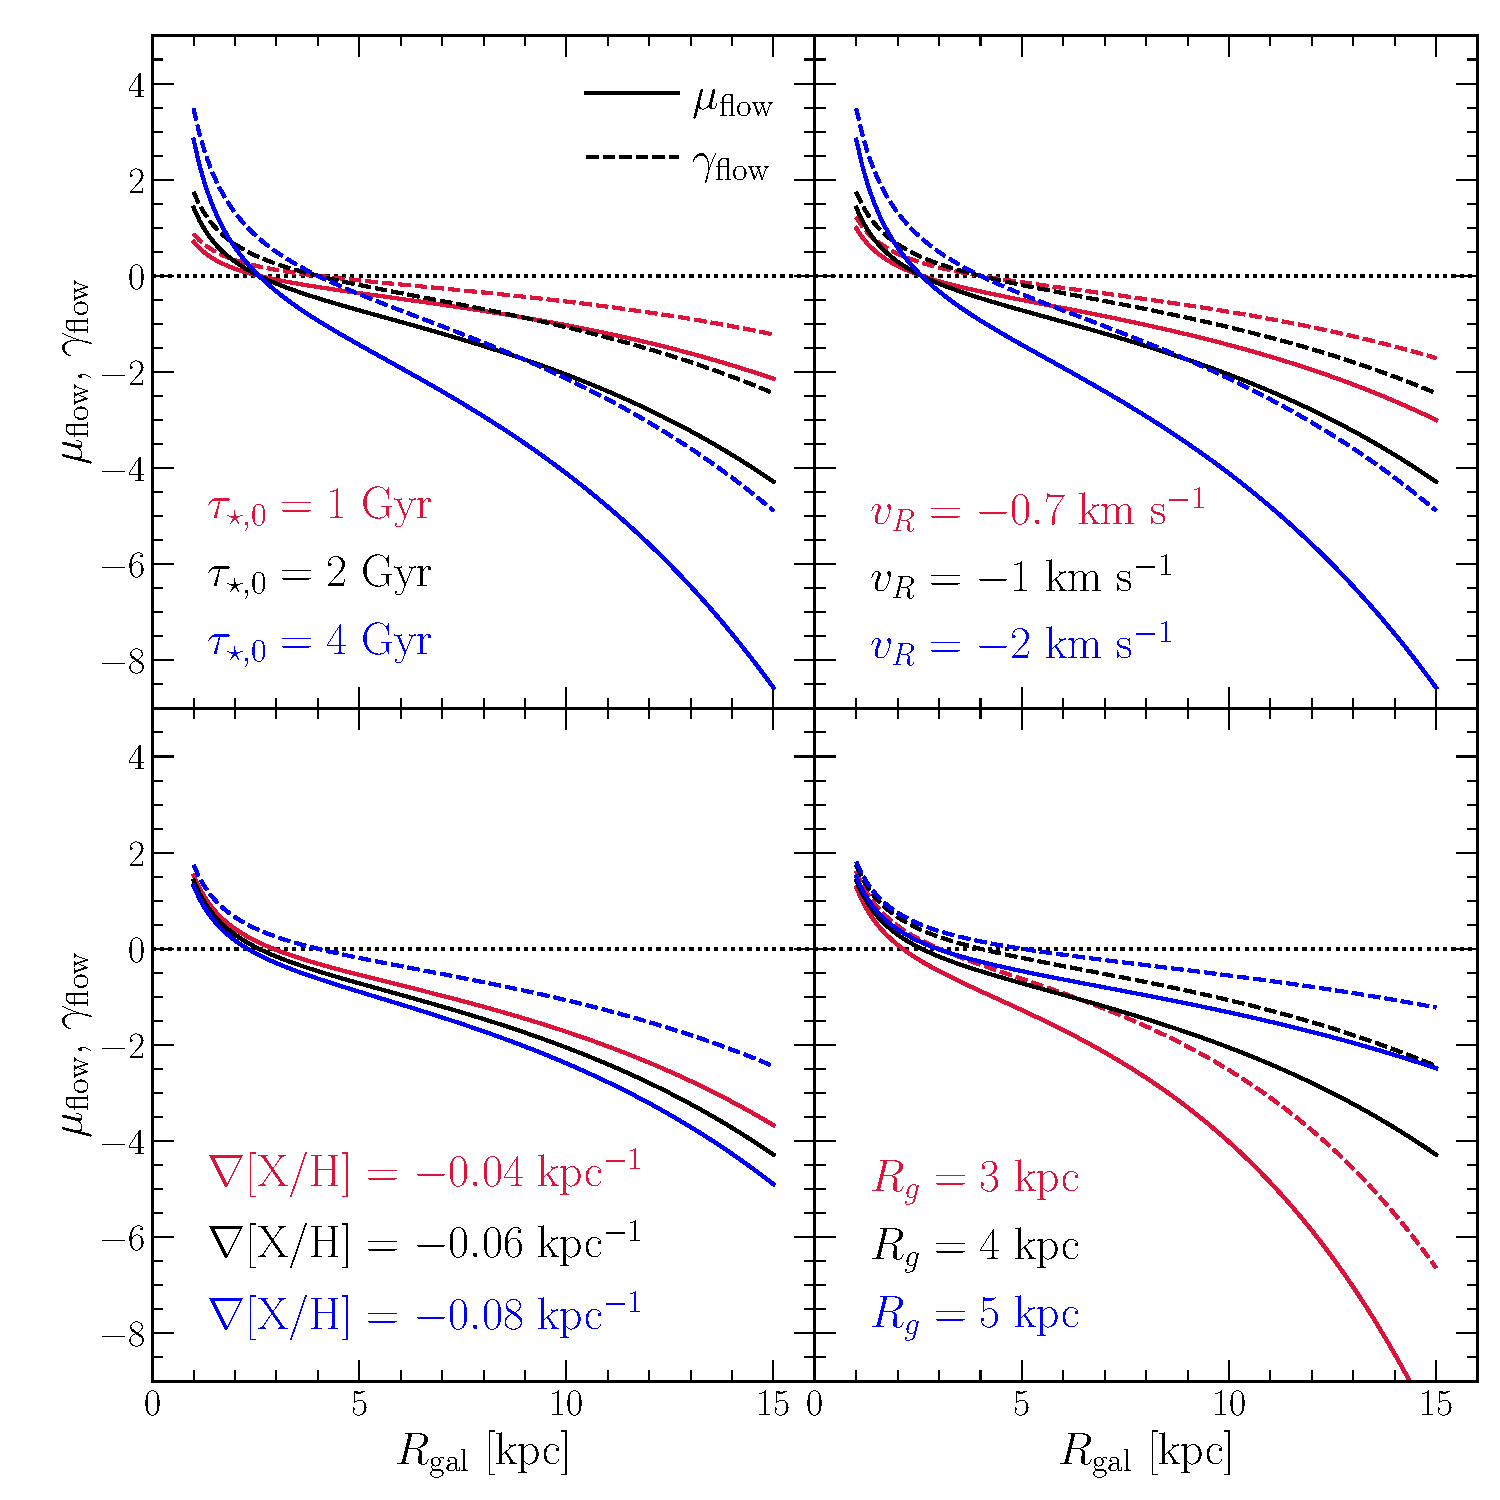
\includegraphics[scale = 0.5]{chapter7/muflow_gammaflow_vs_radius.pdf}
\caption{
The radial flow coefficients~$\mu_\flow$ (solid) and~$\gamma_\flow$ (dashed) as
functions of radius for different parameter choices.
Black lines correspond to the fiducial choice of
($\tau_{\star,0}$,~$v_R$,~\grad{X},~$R_g$) = (2 Gyr, 1 km s$^{-1}$,
$-0.06$ kpc$^{-1}$,~$4$ kpc) and are the same in all panels.
Each panel then shows variations in one of these four parameters according to
the legends in the lower right.
}
\label{outflows:fig:flow-coefficients-vs-radius}
\end{figure*}

\begin{itemize}

	\item $\mu_\flow$ and~$\gamma_\flow$ are parameterized such that radial
	flows are a source if they are positive and a sink if they are negative.
	For an inward gas flow (i.e.,~$v_R < 0$),~$\gamma_\flow > \mu_\flow$.

	\item $0 \leq \gamma_\flow \leq -\tau_\star v_R / R_x$ is an interesting
	region of parameter space in that radial flows are a~\textit{source} of
	gas ($\gamma_\flow > 0$) but a~\textit{sink} of metals ($\mu_\flow < 0$).
	Dilution can be a strong effect in this scenario.

	% \item To understand the impact of radial flows on the metallicity gradient,
	% we must incorporate the effects on both metal and gas masses separately as
	% the metals are affected by the gradient but the gas is not.
	% Isolating the terms~$\dot{M}_{x,\flow}$ and~$\dot{M}_{g,\flow}$:
	% \begin{equation}\begin{split}
	% \dot{Z}_{x,\flow} &= \frac{\dot{M}_x M_g - M_x \dot{M}_g}{M_g^2}
	% \\
	% &= \frac{\dot{M}_x}{M_g} - \left(\frac{M_x}{M_g}\right)
	% \frac{\dot{M}_g}{M_g}
	% \\
	% \dot{Z}_{x,\flow} < 0 \implies \frac{\dot{M}_x}{M_g} &< Z_x
	% \frac{\dot{M}_g}{M_g}
	% \\
	% \frac{\dot{M}_x}{\dot{M}_g} &< Z_x
	% \\
	% \frac{Z_x \dot{M}_\star \mu_\flow}{\dot{M}_\star \gamma_\flow} &< Z_x
	% \\
	% \mu_\flow &< \gamma_\flow.
	% \end{split}\end{equation}
	

\end{itemize}


